\chapter{Classical Statistical Model}

\section{Probability versus statistical inference}

\textbf{Probability theory} begins with a completely specified model which we assume are correct and we compute the probabilities of certain events. 
For example, 
\begin{gather*}
    X_1,\ldots,X_n \overset{iid}{\sim} B(1,\theta)\\
    T = \sum_{i=1}^{n}X_i\sim B(n,\theta)\\
    P(T=t|\theta) = \left( \begin{array}{c} n \\ t \end{array} \right)\theta^t(1-\theta)^{n-t} \quad t=0,1,\ldots,n
\end{gather*}
with $n=20 \to P(T=10|\theta)$ is calculatable if we know $\theta$.
On the other hand, for \textbf{statistical inference}, we observe the realization of certain events,
and using that information we try to infer the probabilistic model that governs the corresponding random experiment. 
For example, $T=10\to$ observed outcome. I want to use this information to make inference about $\theta$.\\

\textbf{Statistical data} result from experiments conducted on a subset of a poopulation, the sample,
and we try to extend the conclusions obtained to the whole population.
\begin{center}
    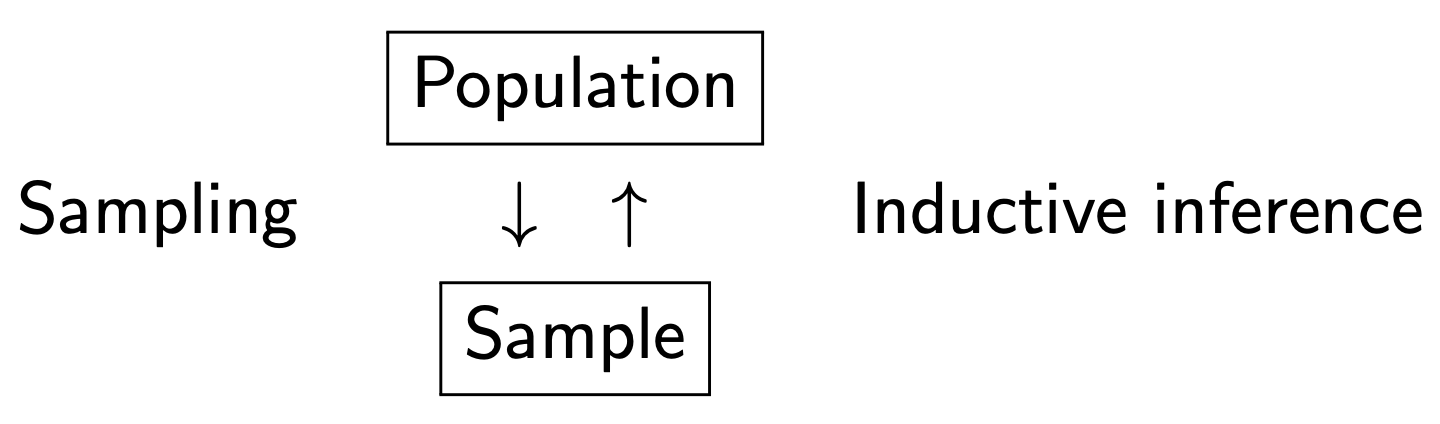
\includegraphics[scale=0.2]{Images/3.png}
\end{center}
\textbf{Inductive inference} means that there is uncertainty regarding the resulting inference.
If we are just drawing finite samples, then we cannot be certain the result is in fact representative of the entire population.
The opposite would be \textbf{deductive inference} where it is of mathematics. No questions about the validity of the inference.
If $A$ holds $\to B$ definitely holds.

\section{Model specification}

To formalize the process of statistical inference.
The characteristic of interest is modeled as a random variable $X$ with cumulative distribution function (cdf) $F$, the statistical model.
The model must be specified either through a \textbf{parametric model} where $F$ is a known up to a finite dimensional parameter, 
e.g. $X$ as normal with mean $\mu$ and variance $\sigma^2$, both unknown.
Or a \textbf{nonparametric model} where $F$ is specified in a nonparametric fashion, e.g. $F$ is an element f the set of all continuous and symmetric distribution.
Focusing on the parametric statistical model:
\begin{equation*}
    \mcF = \{F(\cdot|\theta):\underbrace{\theta}_{\text{parameter}}\in\underbrace{\Theta}_{\text{parameter space}}\}
\end{equation*}

\ex[]{Application : daily return of financial asset}{
    We can propose a normal $\to$
    $\mcF = \{N(\mu,\sigma^2):\mu\in\bbR,\sigma >0\}$
    or a gamma $\to$
    $\mcF = \{G(\alpha,\lambda):\alpha,\lambda >0\}$
}
\ex[]{Application : insurance policy}{
    If we are interested in the number of claims per year in an insurance policy, we can propose the Poisson
    $\to\mcF = \{Po(\lambda):\lambda >0\}$
}

The specificiation is important and results from many factors, namely based on the knowledge of the problem at hand, knowledge of previous studies, and knowledge of probability theory.
The consequence of model misspecification is always negative but is smaller for larger samples.

\subsection{Sampling}

\textbf{Random sampling} means that the observed data are one of many possible data sets we could have obtained in the same circumstances.
The set of $n$ observations, $(x_1,\ldots,x_n)$ which we have observed is a realization of an $n$-dimensional random variables $(X_1,\ldots,X_n)$.
\begin{equation*}
    \begin{split}
        (X_1,\ldots,X_n) & \qquad\text{Random sample}\\
        (x_1,\ldots,x_n) & \qquad\text{Observed sample}
    \end{split}
\end{equation*}
The \textbf{sample space} is a subset of $\bbR^n$ that contains the set of possible values for $x_1,\ldots,x_n$. We denoteit by $\mcX$.

\dfn[]{IID random sampling}{
    When the $n$ random variables that compose the random sample are
    \begin{itemize}
        \item mutually independent $\to x_i\ind x_j | \theta$
        \item identically distributed, with the same distribution as $X\to x_i\sim x_j | \theta$
    \end{itemize}
    we say that $(X_1,\ldots,X_n)$ constitutes an iid random sample of size $n$ obtained from the population $X$.
    In notation, $X_1,\ldots,X_n|\theta\overset{iid}{\sim}X$, $X$ follows the common distribution of all $x_i$'s, $x_i\sim X$.
}
If $\mcF = \{f(\cdot|\theta):\theta\in\Theta\}$ and $X_1,\ldots,X_n|\theta\overset{iid}{\sim} X$, then
\begin{equation*}
    \begin{split}
        F_{X_1,\ldots,X_n}(x_1,\ldots,x_n|\theta) & =\prod_{i=1}^{n}F_{X_i}(x_i|\theta)\qquad\text{by independence}\\
        & = \prod_{i=1}^{n}F(x_i|\theta)\qquad\text{since }X_i\sim X 
    \end{split}
\end{equation*}
and similarly for the probability density function
\begin{equation*}
    f(x_1,\ldots,x_n|\theta)=\prod_{i=1}^{n}f(x_i|\theta)
\end{equation*}
\begin{proof}
    \textbf{Poisson distribution}
    \begin{equation*}
        \begin{split}
            f(x_1,\ldots,x_n|\lambda) & = \prod_{i=1}^{n}f(x_i|\lambda)\\
            & = \prod_{i=1}^{n} e^{-\lambda}\frac{\lambda^{x_i}}{x_i!}\\
            & = P(x_1 = x_1,\ldots,x_n = x_n|\lambda)\\
            & = e^{-n\lambda}\frac{\lambda^{\sum_{i=1}^{n}x_i}}{\prod_{i=1}^{n}x_i!}\to\text{Annex 1}
        \end{split}
    \end{equation*}
    Annex 1: 
    \begin{itemize}
        \item $e^a e^b = e^{a+b}$
        \item $a^x a^y = a^{x+y}$
    \end{itemize}
\end{proof}

\section{Statistics}

\dfn[]{Statistic}{
    A statistic is any function of $(X_1,\ldots,X_n)$ that does not depend on unknown parameters.
}
\ex[]{Statistic}{
    In the context of a $N(\mu,\sigma^2)$, $\mu\in\bbR$ and $\sigma>0$ unknown.\\

    \textbf{Uni-dimensional} statistics include
    \begin{itemize}
        \item $T = \sum_{i=1}^{n}X_i$
        \item $\bar{X}=\frac{1}{n}T$
        \item $S^2 = \frac{1}{n}\sum_{i=1}^{n}(X_i-\bar{X})^2$
    \end{itemize}
    \textbf{Bi-dimensional} statistics include
    \begin{itemize}
        \item $(T, \sum_{i=1}^{n}X_i^2)$
        \item $(\bar{X},S^2)$
    \end{itemize}
}
\ex[]{Not statistic}{
    \begin{equation*}
        \sum_{i=1}^{n}(X_i-\mu)^2\qquad \frac{1}{\sigma^2}\sum_{i=1}^{n}X_i^2
    \end{equation*}
    are not statistics becuase they depend on unknown parameters. If $\sigma^2$ is known, then $\frac{1}{\sigma^2}\sum_{i=1}^{n}X_i^2$ is a statistic.
}

Statistics operate a data reduction and are summaries of the information contained in the random sample. 
Statistics are random variables, as usual, it is important to distinguish between the random variable and its observed value.
\begin{center}
    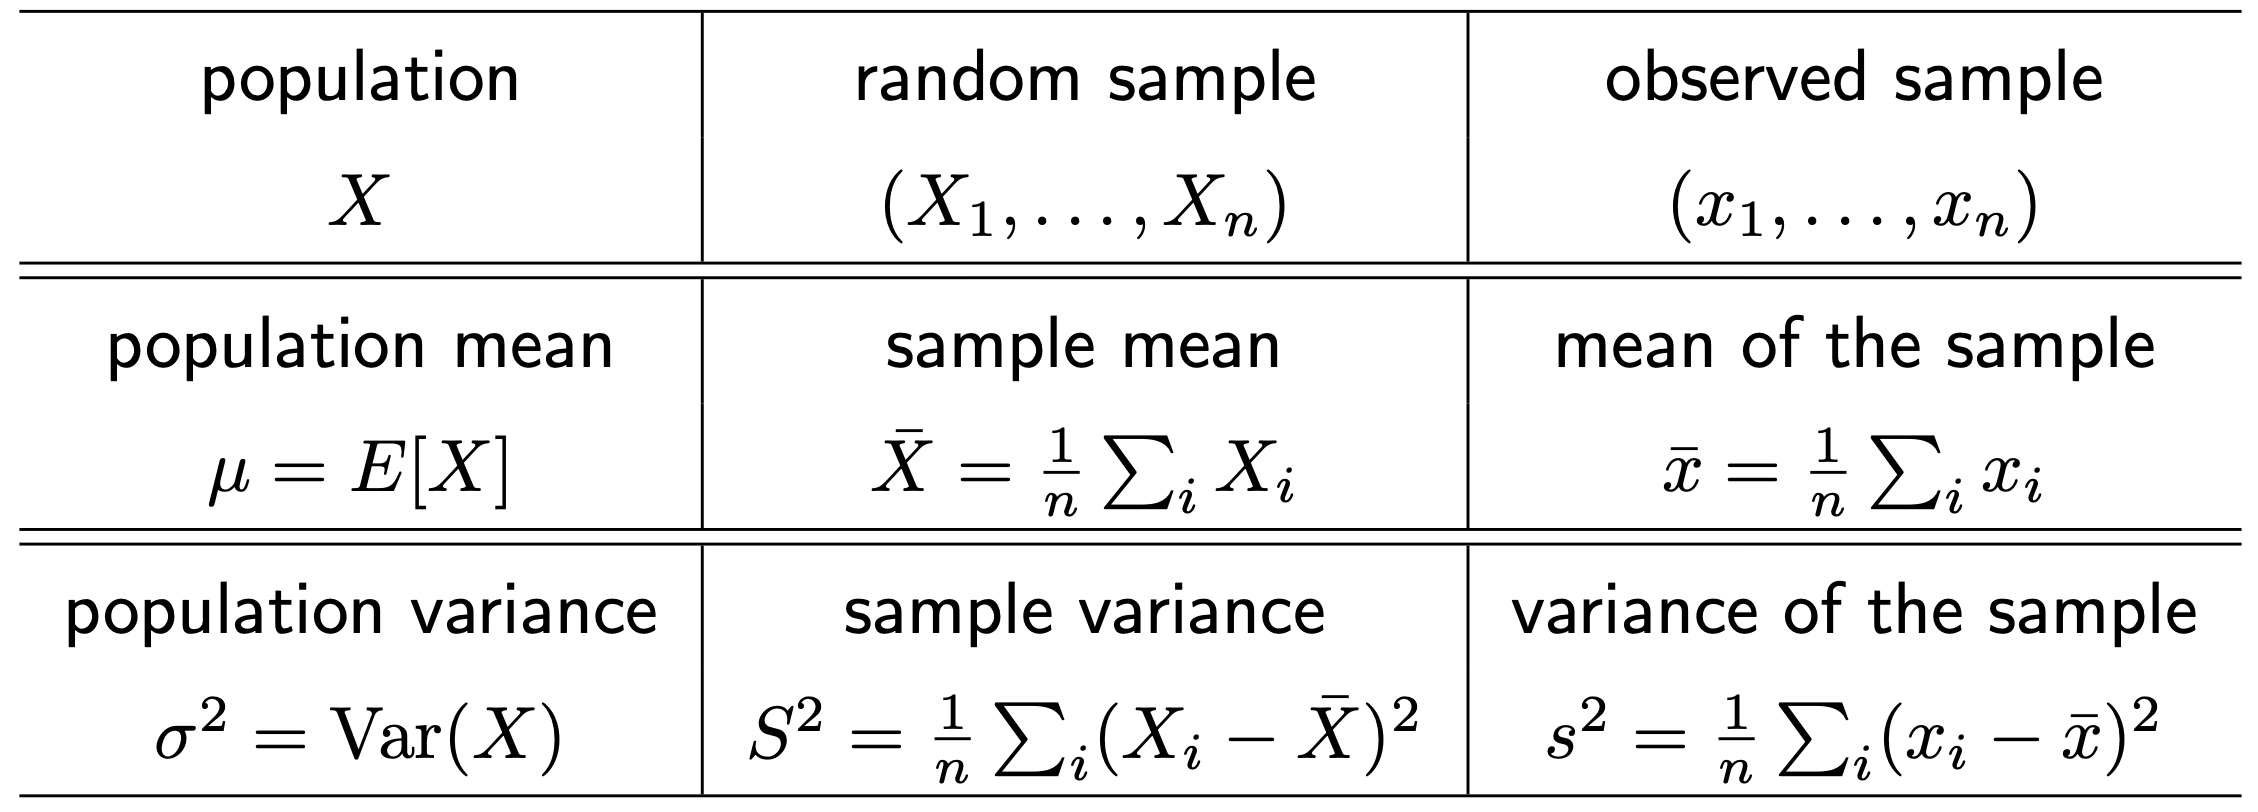
\includegraphics[scale=0.2]{Images/4.png}\\
    Probability vs. Statistics vs. Data exploration
\end{center}

\section{Sampling distribution}
\begin{itemize}
    \item Definition
    \item Methods to obtain the sampling distribution of a statistic
        \begin{itemize}
            \item Monte Carlo simulation
        \end{itemize}
    \item Sample distribution of the sample moments
        \begin{itemize}
            \item Sample moments
            \item Properties of the sample mean
            \item Properties of the sample variance
            \item Properties of the bias-corrected sample variance
            \item Properties of central sample moments
            \item Asymptotic distribution of $\bar{X}$
        \end{itemize}
    \item Order statistics
\end{itemize}